%%%%%%%%%%%%%%%%%%%%%%%%%%%%%%%%%%%%%%%%%
% University Assignment Title Page 
% LaTeX Template
% Version 1.0 (27/12/12)
%
% This template has been downloaded from:
% http://www.LaTeXTemplates.com
%
% Original author:
% WikiBooks (http://en.wikibooks.org/wiki/LaTeX/Title_Creation)
%
% License:
% CC BY-NC-SA 3.0 (http://creativecommons.org/licenses/by-nc-sa/3.0/)
% 
% Instructions for using this template:
% This title page is capable of being compiled as is. This is not useful for 
% including it in another document. To do this, you have two options: 
%
% 1) Copy/paste everything between \begin{document} and \end{document} 
% starting at \begin{titlepage} and paste this into another LaTeX file where you 
% want your title page.
% OR
% 2) Remove everything outside the \begin{titlepage} and \end{titlepage} and 
% move this file to the same directory as the LaTeX file you wish to add it to. 
% Then add \input{./title_page_1.tex} to your LaTeX file where you want your
% title page.
%
%%%%%%%%%%%%%%%%%%%%%%%%%%%%%%%%%%%%%%%%%
%\title{Title page with logo}
%----------------------------------------------------------------------------------------
%	PACKAGES AND OTHER DOCUMENT CONFIGURATIONS
%----------------------------------------------------------------------------------------

\documentclass[12pt]{article}
\usepackage[english]{babel}
\usepackage[utf8x]{inputenc}
\usepackage{amsmath}
\usepackage{graphicx}
\usepackage[colorinlistoftodos]{todonotes}

\begin{document}

\begin{titlepage}

\newcommand{\HRule}{\rule{\linewidth}{0.5mm}} % Defines a new command for the horizontal lines, change thickness here

\center % Center everything on the page



\includegraphics{logo.png}\\[.1cm] % Include a department/university logo - this will require the graphicx package

%----------------------------------------------------------------------------------------
%	HEADING SECTIONS
%----------------------------------------------------------------------------------------

\text{\LARGE Department of Computer Science and Engineering}\\[1.5cm] % Name of your university/college

%
\textsc{\Large Report on }\\[0.5cm] % Major heading such as course name
%----------------------------------------------------------------------------------------
%	TITLE SECTION
%----------------------------------------------------------------------------------------

\HRule \\[0.4cm]
{ \huge \bfseries ARA – The Ant-Colony Based Routing Algorithm for MANETs}\\[0.4cm] % Title of your document
{Mesut G¨unes, Udo Sorges, Imed Bouazizi}
\HRule \\[1cm]
 
%----------------------------------------------------------------------------------------
%	AUTHOR SECTION
%----------------------------------------------------------------------------------------

\begin{minipage}{0.5\textwidth}
\begin{flushleft} \large
\emph{Report Writers:}\\
Shantanu Sarkar\newline(0416052041) \newline % Your name
Mahmud Ahmed\newline(0416052027) \newline
Md. Mostafizur Rahman\newline(0416052032) 
\end{flushleft}
\end{minipage}
~
\begin{minipage}{0.4\textwidth}
\begin{flushright} \large
\emph{Supervisor:} \\
Dr. Ashikur  Rahman% Supervisor's Name
\end{flushright}
\end{minipage}\\[1cm]



% If you don't want a supervisor, uncomment the two lines below and remove the section above
%\Large \emph{Author:}\\
%John \textsc{Smith}\\[3cm] % Your name

%----------------------------------------------------------------------------------------
%	DATE SECTION
%----------------------------------------------------------------------------------------

{\large \today}\\[.5cm] % Date, change the \today to a set date if you want to be precise

%----------------------------------------------------------------------------------------
%	LOGO SECTION
%----------------------------------------------------------------------------------------


 
%----------------------------------------------------------------------------------------

\vfill % Fill the rest of the page with whitespace

\end{titlepage}

\tableofcontents

\newpage
\begin{abstract}

\end{abstract}

\section{Introduction}
Introduction of the report goes here. 


\section{Context and Problem Statement}


\section{Idea}

\section{Evaluation Metrics}
According to the Authors, the main feature of ARA is its low routing overhead and easy maintainability of routes between nodes in the topology. So, The evaluation metrics considered to measure the performance of ARA are:
\begin{itemize}
\item Delivery rate 
\item Routing overhead in terms of bits
\item Routing overhead in terms of packets
\end{itemize}

\section{Evaluation Process}
The performance of ARA was evaluated using simulation in terms of evaluation metrics mentioned earlier. 
The simulation was implemented in ns-2. Some important parameters of the simulation environment are:

\begin{itemize}
\item Simulation area  1500m×300m 
\item Maximum velocity of nodes 10 m/s using Random waypoint model.
\item Simulation time  900 seconds
\item 10 Constant bit rate(CBR) connections
\item 7 different pause times\footnote{pause time indicates the mobility of the nodes} 0,30, 60, 120, 300, 600 and 900 seconds
\end{itemize}


\section{Evaluation Results}
Multiple simulations were run and the results were collected for evaluation. 
\subsection{Comparison with existing routing protocols in delivery rate}
The best way to evaluate the performance of a new algorithm is to compare the performance with the existing algorithms. So, the performance of ARA was compared with AODV,DSR and DSDV in terms of delivery rate. The observed results are shown in Figure~\ref{fig:picture1}. With high mobility both DSR and ARA has more than 95\% delivery rate. 
Throughout the simulations ARA performed better than DSDV and AODV in this criteria. Figure~\ref{fig:picture2} shows the delivery rate of ARA within the confidence interval of 95\%. As we can see All results are above 85\% and most results are within the range 90\% and 100\% throughout the 10 simulation runs.


\begin{figure}[t!]
\centering
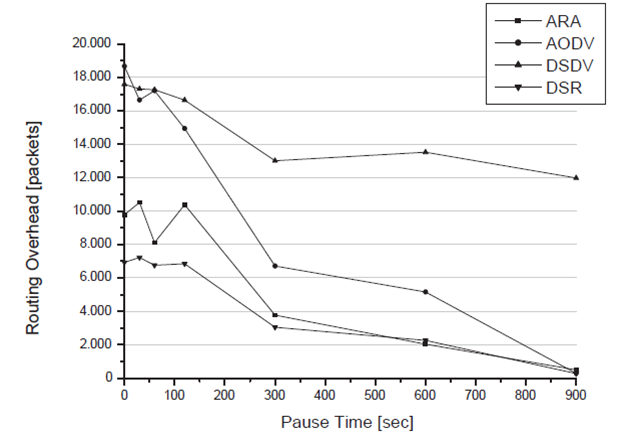
\includegraphics[width=0.7\textwidth]{Picture1.png}
\caption{\label{fig:picture1}Successful delivered packets as a
function of pause time.}
\end{figure}


\begin{figure}[t!]
\centering
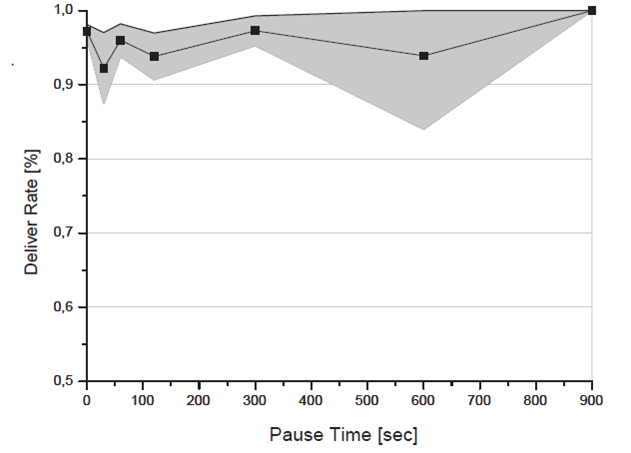
\includegraphics[width=0.7\textwidth]{Picture2.png}
\caption{\label{fig:picture2}Delivery rate of ARA. Confidence interval of 95\%}
\end{figure}


\subsection{Routing Overhead Comparison}
As different protocols generate the overhead in very different ways, the routing overhead of different algorithms were observed both in terms of fraction of routing packets needed to deliver a data packet and fraction of databits needed for routing.
\subsubsection{Routing Overhead in terms of databits}
Figure ~\ref{fig:picture3} shows the routing overhead of routing algorithms in term of routing bit as a fraction of total databits. In this case ARA give the best results throughout the simulations. Figure ~\ref{fig:picture4} show the overhead of ARA in 95\% confidence interval.
  
\begin{figure}[t!]
\centering
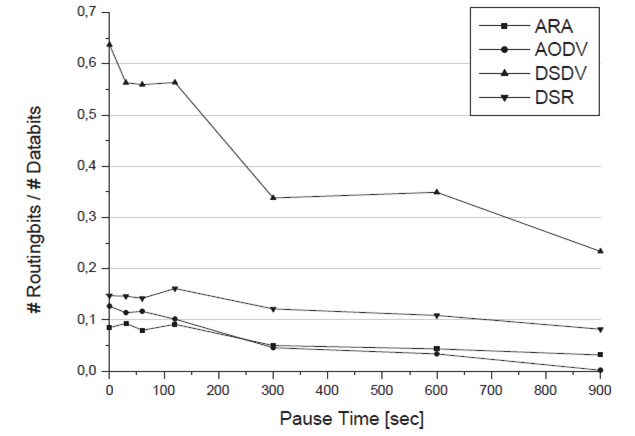
\includegraphics[width=0.7\textwidth]{Picture3.png}
\caption{\label{fig:picture3}Pause time vs Fraction of successfully send bits and the needed bits}
\end{figure}

\begin{figure}[t!]
\centering
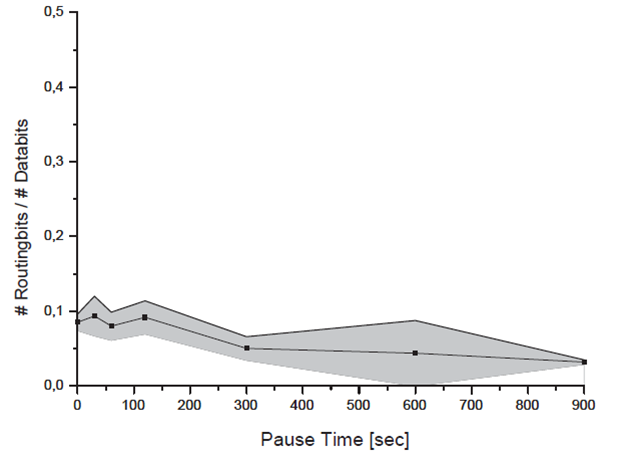
\includegraphics[width=0.7\textwidth]{Picture4.png}
\caption{\label{fig:picture4}Overhead of ARA in bits. Confidence interval of 95\%}
\end{figure}



\subsubsection{Routing Overhead in terms of packets}
Figure ~\ref{fig:picture5} shows the routing overhead of routing algorithms in term of packets. In this case ARA give second best results following DSR.This is due to the needed flooding of the approach in the route finding phase. With high node mobility route failure occur more often, thus requires the
performing of the route failure handling part of the algorithm,which in worst case has to backtrack the path until
the sender. Figure ~\ref{fig:picture6} show the overhead of ARA in 95\% confidence interval.
  
\begin{figure}[t!]
\centering
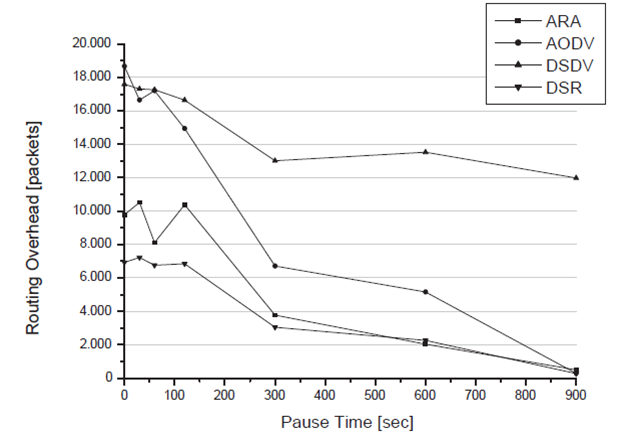
\includegraphics[width=0.7\textwidth]{Picture5.png}
\caption{\label{fig:picture5}Pause time vs Fraction of successfully send bits and the needed bits}
\end{figure}

\begin{figure}[t!]
\centering
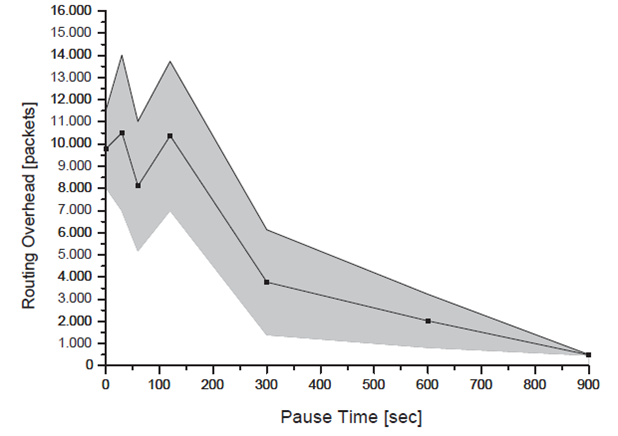
\includegraphics[width=0.7\textwidth]{Picture6.png}
\caption{\label{fig:picture6}Overhead of ARA in packets. Confidence interval of 95\%}
\end{figure}


\textbf{Remarks:} ARA is a good choice for mobile networks in terms of data delivery,routing overhead. But a better conclusion can be derived if individual performances of DSR,DSDV,AODV were presented in 95\% confidence interval like Figure ~\ref{fig:picture2}, Figure ~\ref{fig:picture4}, Figure ~\ref{fig:picture6}. In that case we would be able to observe the fluctuations of performance over different mobility. 
Nevertheless, we consider ARA as a robust and highly maintainable routing protocols in mobile adhoc networks. 

\section{Limitations of ARA}


\section{Future Works}

\section{Conclusion}

\end{document}